\chapter{定界搜索}

\section{组合优化问题}

在归约一章中,我们介绍了著名的NP-完全问题:CNF-SAT。SAT是大量问题的一般形式,因此在实际中被广泛应用。然而SAT solver也有其局限:
SAT是一个判定问题,当我们试图把很多常见的问题如最大团(Clique)、最小集合覆盖(Set Cover)等问题归约到判定版本的SAT时,困难就出现了。
这些问题都有共同的形式:它们都属于组合优化问题。组合优化问题通常是要在一个离散的集合中求解满足一定约束条件的最优解,而不仅仅是判定满足约束条件的解是否存在。

相应的,SAT问题也有其推广版本:带权Max-SAT。如果我们给SAT问题中的每个布尔变量$x_i$一个权值$W_i$,并且求满足$C = C_1 \land C_2 \land \ldots \land C_n$赋值
中权值最大的那个:
$$
\begin{array}{cl}
\displaystyle \argmax_{x} & \displaystyle \sum_{i\in V} W_i,\ \textrm{其中}\ V = \{i~|~x_i = T\} \\
\textrm{subject to} & C(x) = T \\
\end{array}
$$

可想而知,带权Max-SAT问题的求解比SAT要困难得多,相应能够求解问题的规模也比SAT solver小得多。
所以,当我们面对NP-难的优化问题时,机械地把它归约到带权Max-SAT有时并不能满足我们的需求。我们需要从问题自身的结构出发
设计有针对性的求解算法。

遗传算法和模拟退火算法常用于约束条件不强而解空间非常大的搜索问题。这类算法的特点是通常可以在很短的时间内就得到一个相当好的解,
但大部分时候却很难回答何时收敛以及是否收敛到全局最优解这个问题。它们的应用场景通常是并不需要精确最优解的规模巨大的组合优化难问题。

\section{搜索与图遍历}

\section{估界与剪支}

我们假设状态空间是一个非负权有向图$G(V, E, W)$,而我们需要在$G$中搜索$s$到$t$的最短长度路径,路径
$v_1, v_2, \ldots, v_m$的长度定义为$\sum_{i=2}^{m} W_{v_{i-1}, v_i}$。
非负权值的假设隐含了随着搜索过程的深入,路径的长度总是单调增加的,绝大多数搜索问题都满足这样的性质。

如果我们已经到达了状态空间的中的某个点$v$, 且路径$s\rightsquigarrow v$的长度为$\ell$。此时,若我们知道
一个$v\rightsquigarrow t$的最短路径长度为$h$,则可以立即得到结论:$s\rightsquigarrow v\rightsquigarrow t$
能够生成一个长度是$\ell + h$的解,并可以立即终止搜索(因为我们已经找到了$s\rightsquigarrow v\rightsquigarrow t$
的最短路径)。

在现实中,得到$h$的精确数值是不现实的(否则我们就完全不需要搜索了)。但我们通常可以对$h$的大小作一个估计,
记为$\hat{h}$。如果对于所有的$v$,都有$\hat{h}\le h$,则我们称估计$\hat{h}$是真值$h$的一个下界。
下界的性质对于搜索剪支是非常重要的,我们在之后都假设$\hat h$具有这样的性质。
如果当前已经搜索到一条长度是$L$的路径,则当$\ell + \hat{h} \ge L$时,由于$h\ge \hat{h}$,我们有
$$\ell + h \ge L$$总是成立,即从$v$开始的任何路径,都不可能产生一个比当前候选解更优的解,对$v$的搜索可以立即终止。

更直观地说,$\hat h$的含义是``从当前结点到目标至少需要的距离'',而剪支的条件则表达为
``如果从当前结点出发,无论如何也无法产生最优解,则应当立即终止当前搜索的分支''。需要强调的是,
$\hat h$必须是当前结点到目标结点
的一个下界。我们用贪心等策略求得的一个较优解通常是不能作为下界使用的,相反,较优解是$h$的一个
上界($h$绝不可能比一个最优性未知的可行解大),而我们寻找的$\hat h$则必须在任何情况下都小于$h$。

\medbreak

虽然$\hat h$必须根据问题本身的性质来设计,为问题估计一个好的下界通常是十分困难的。
但考虑我们总是比较当前结点到目标结点的估计$\ell + \hat h$和当前最优解$L$的数值,
为了提高搜索的效率,即便不考虑问题的结构,我们也有一些基本思想指导优化:

\begin{enumerate}
 \item 我们希望$\ell+\hat{h}$尽可能的大,也就是希望让$h$的估计尽可能大。一个策略是可以用不同的算法计算$h$的多个下界
   $\hat h_1, \hat h_2, \ldots, \hat h_k$,并取其中最大的那个作为一个``更精确''的下界,
   即$\hat h= \max\{ \hat h_1, \hat h_2, \ldots, \hat h_k\}$。
   
   另一个常用的技巧类似于双向搜索:我们可以从目标结点$t$出发,求出一定数量的结点到$t$的最短路径。这使得在搜索的最后几层,
   我们总是能够使用完全精确的下界($\hat h=h$),从而提高搜索的效率。
 \item $\ell + \hat{h}$的数值是跟``当前最优解''\ $L$进行比较的,因此我们希望$L$尽可能小(即尽可能接近最优解)。
   一个合理的策略是,我们可以用一个错误的贪心或动态规划求出一个$s$到$t$的合法路径(但未必是最优的),并用该路径作为初始解,
   从而能够减少算法早期在无用分支上的尝试。
   
   此外,由于我们希望$L$能尽量的小,在基于DFS的搜索中,
   我们应当优先尝试那些``有前途''的分支,尽可能早地获得一个更好的解,这就是搜索顺序的问题。
   有时我们可以优先搜索$\hat{h}$较小的分支,因为$\hat{h}$很多时候是$h$数值的一个反映,但这样的技巧需要结合$\hat{h}$的性质
   谨慎使用。
\end{enumerate}

著名的${\rm A}^*$算法就是上述这些策略的一个综合:类似于Dijkstra最短路径算法,${\rm A}^*$算法每次选择一个结点扩展
其相邻结点。
与Dijkstra算法不同的是,${\rm A}^*$算法并不选取距离最短的结点,而是选取$\ell + \hat h$最小的结点进行扩展。
Dijkstra算法可以看作是$\hat h=0$的${\rm A}^*$算法。
在使用优先队列实现${\rm A}^*$算法时需要特别注意的是,若估计函数$\hat h$不满足单调性
$\hat h(u)\le d(u, v) + \hat h(v)$,我们将不能使用状态空间的重复消除算法。
使用${\rm IDA}^*$时我们没有考虑重复状态的搜索,因此也自然避免了这个问题。

我们用一个例子来说明上述这些优化策略的使用:

\begin{prob}[01背包]
 有$n$个物品,每个物品$i$都有其价值$V_i$和重量$W_i$,求解如下的整数线性规划问题:
 $$\begin{array}{rl}
  {\rm maximum}     & \sum_{i=1}^n V_i\cdot x_i \\
  {\rm subject\ to} & \left( \sum_{i=1}^n W_i\cdot x_i \right) \leq W \\
                   & x_i \in \{0, 1\}\\
   \end{array}
 $$
 该问题的直观含义是,我们有一个能够承受$W$重量的背包,
 如何选择放入哪些物品放入背包,在不超过背包重量限制的前提下,装走价值总和最大的物品?
\end{prob}

\begin{solution}
 我们可以很容易地设计一个搜索算法,按顺序搜索每一个物品是否放入背包。
 我们搜索的每一个状态,都是若干个物品已经确定了放入或没有放入背包中,剩下的物品可以任意处理,
 如图~\ref{fig:knapsack_tree} 所示。

 \begin{figure}[h]
 \center
 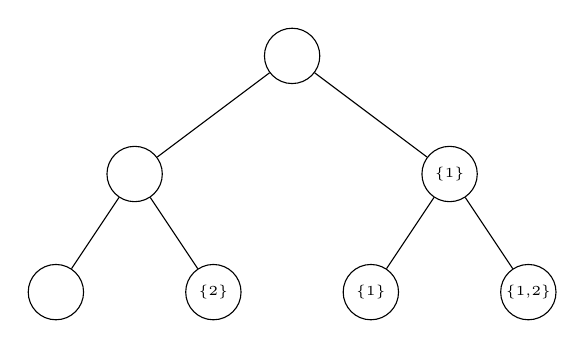
\begin{tikzpicture}[level/.style={sibling distance=40mm/#1}]
 \node [circle,draw,minimum size=20pt,inner sep=0pt] (z){$\varnothing$} 
  child {node [circle,draw,minimum size=20pt,inner sep=0pt] (a) {$\varnothing$}
   child {node [circle,draw,minimum size=20pt,inner sep=0pt] (b) {$\varnothing$}}
   child {node [circle,draw,minimum size=20pt,inner sep=0pt] (c) {$\scriptscriptstyle \{2\}$} }
  }
  child {node [circle,draw,minimum size=20pt,inner sep=0pt] (d) {$\scriptscriptstyle\{1\}$}
   child {node [circle,draw,minimum size=20pt,inner sep=0pt] (e) {$\scriptscriptstyle\{1\}$} }
   child {node [circle,draw,minimum size=20pt,inner sep=0pt] (f) {$\scriptscriptstyle\{1,2\}$} }
  };
 \end{tikzpicture}
 \caption{背包问题的搜索树}
 \label{fig:knapsack_tree}
\end{figure}


 朴素的搜索总共会生成$2^n$个搜索树叶子结点,我们必须在适当的时候剪支以提高搜索的效率,
 为此就必须设计一个好的估计函数$\hat{h}$。注意到我们的优化目标是最大化物品的价值,因此我们的$\hat h$应当是
 物品价值的一个上界(剪支的直观含义是,如果包内物品的价值加上剩下物品装入背包所能获得价值的上界仍然不能超过当前
 最优解)。

 假设在搜索的某个中间状态,剩下的物品集合为$S$,背包还能够容纳的重量是$W'$,我们的目标是为这个01背包问题
 寻找一个上界。在寻找上界的过程中,我们经常使用优化问题的松弛技术(这也是设计近似算法的一个常用技巧)。
 如果我们将$x_i\in\{0,1\}$的条件放松为$0\le x_i\le 1$,则整数线性规划就被转换成了一个线性规划:
 $$\begin{array}{rl}
  {\rm maximum}     & \sum_{i\in S} V_i\cdot x_i \\
  {\rm subject\ to} & \left( \sum_{i\in S} W_i\cdot x_i \right) \leq W' \\
                   & 0\leq x_i \leq 1\\
   \end{array}
 $$
 若上述线性规划的最优解为$\hat h_1$,则$\hat h_1\ge h$总是成立,
  我们可以保证松弛后优化问题的最优解是原问题的一个上界。
 松弛问题的直观解释是,放松每个物品要么放入背包,要么不放入背包
 的限制,每个物品都可以任意拆分,拆分后的价值与拆分部分的重量成正比。而可拆分背包也无需使用线性规划求解:
 只需将物品按照性价比$V_i / W_i$从大到小排序,并按顺序放入背包即可。

 我们还可以设计其他的估计函数,例如我们可以引入双向搜索的概念,在所有物品中选出一个子集$K$,
 枚举$K$中所有子集合$F\subseteq K$的重量和价值。这样,我们就能够得出只使用$K$中的物品,
 在背包剩余$w$容量时,所能获得的最大价值$f(w)$。在搜索到最后几层时,我们就可以直接使用二分查找
 求得精确的$h$,从而无需再搜索下去,即
 $$\hat h_2 = \begin{cases}
  f(W'), & S = K; \\
  +\infty,    & S\neq K.
  \end{cases}
 $$

 综合两个不同的估计函数,我们可以取它们中较小的那个作为更精确的上界:
 $$\hat h=\min \big\{\,\hat h_1, \hat h_2\,\big\}.$$

 最后我们确定搜索的顺序。从一般意义来说,优先搜索那些性价比高的物品,以及优先进入$\hat{h}$高的分支
 有利于较早获得最优解,但这并不是绝对的,甚至有时是很糟糕的。
 为了达到最佳的搜索效果,我们也许需要针对不同的问题实例设计不同的搜索顺序。
\end{solution}


\subsection{设计估计函数}

如果我们有一个近似比为$\alpha$的近似算法,求得一个解为$X$。根据近似算法的性质,我们知道$X \leq \alpha {\it OPT}$,
也就得到原问题的一个下界
$$\hat h = {1\over \alpha}X \leq {\it OPT}.$$

将近似算法作为下界的估计有一个问题:很多近似算法的性能非常之好,以至于在实际情况下与最优解相差无几。一旦除以近似比,下界的估值就显得相当小了。
而为了体现启发函数的作用,我们希望下界估计得尽可能大,例如如果我们得到了问题的一个$({\it OPT}+1)$-近似算法,
则${\it OPT}\le X\le {\it OPT}+1$,取
$\hat h=X-1$,则
$${\it OPT}-1 \le \hat h \le {\it OPT}$$
是一个非常精确的估计,能够很有效地增加搜索的效率。

\begin{prob}[比较排序]
 我们知道任何基于比较的排序算法,为了排序5个数,在最坏情况下都需要7次比较。
 如果我们给定$n$个数(假设它们互不相同),并且已知其中一些的大小关系(例如第3个数大于第4个数),
 问将它们排序至少还需要比较多少次?
\end{prob}

\begin{solution}

给定一个偏序,它可能所有全序的数量$t$
$O(n^2\cdot 2^n)$的基于状态压缩的动态规划。
我们知道,任何排序算法都不可能在少于$\lceil \log_2 t\rceil$次比较之内将偏序转换为全序
(因为$k$次比较至多只能区分$2^k$种不同的情况),因此$\lceil \log_2 t\rceil$
是将当前状态偏序确定为全序比较次数的一个下界。

\end{solution}
